

\chapter{Исчисление остатков}

\vrezka{
Покончив с движениями, мы снова погружаемся в алгебру целых чисел и приступаем к изучению остатков (вычетов).

Арифметика вычетов дает богатый фактологичекий материал для изучения свойств простых чисел, а также позволяет по-новому взглянуть на операции Минковского с числовыи множествами и выйти на такие важные вехи теории множеств, как виды отношений и фактормножества.
}

\section{Арифметика остатков}

\subsection{Конспект}
\begin{enumerate}\setlength{\itemsep}{1pt}
\item Рассмотрим бытовую задачу. Вам нужно выключить печку через 40 минут, но у вас нет таймера, зато есть будильник, на котором можно выставить время звонка. Сейчас 12:30, на какое время требуется поставить будильник? Ответ: 13:10. Почему так? Дело в том, что в часе 60 минут, и если к 30 минутам прибавить 40, получается 70 минут, что больше часа. Поэотму добавляем 1 час и остаток --- 10 минут.
\item Еще пример: сколько часов будет через 20 часов, если сейчас 8 утра? Можно решать аналогично: $8+20=28$, затем убираем полные сутки, т.е. 24 часа, остается 4 часа утра.
\item Можно решать иначе. 20 часов --- это $-4$ часа от суток. Следовательно, нужно просот вычесть из 8 утра 4 часа и получим те же 4 часа утра.
\item Во всех случаях мы решаем задачу нахождения остатка от деления на некоторое число. В случае минут это 60, в случае часов это 24.
\item Когда вас просят отметить в анкете количество полных лет, то вам по сути нужно найти неполное частное от деления вашего возраста на 1 год. Конечно, в данном случае нам это просто сделать, т.к. каждый год мы запоминаем именно количество прожитых лет, а не дней или недель.
\item Но, например, во многих сферах деятельности планирование календаря происходит неделями (и даже у себя в компьютере в настройках календаря вы можете вывести номер текущей недели в году). А сколько недель в году? Для этого нужно найти неполное частное от деления 365 (или 366) на 7, оно составляет 52.
\item Остаток от деления на неделю есть число от 0 до 6, которое определяет сдвиг вперед относительно текущего дня недели. Например, если сегодня четверг, то какой день недели будет через 30 дней? Мы выбрасываем из 30 4 полных недели, что составляет 28 дней, и находим остаток, который равен 2. Это значит, что через 30 дней будет четверг плюс 2 дня, т.е. суббота.
\item Точно так же можно легко заметить, что каждый год происходит смещение дат на 1 или два дня вперед относительно дней недели. Так, если в этом году 1 января было средой, то в следующем оно будет или четвергом (если мы не переходим через 29 февраля), или пятницей (если текущий год --- високосный, т.е. содержит 366 дней), как на картинке ниже.

\begin{center}
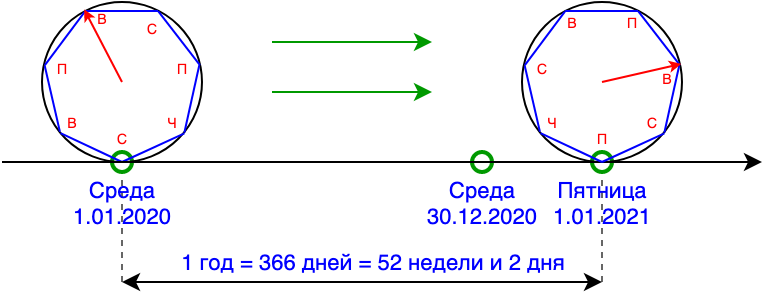
\includegraphics[scale=0.4]{weekdays.png}
\end{center}

\item Каждые 28 лет (а 28 --- это наименьшее общее кратное 7 и 4) соответствие дат и дней недели повторяется.
\item При расчетах на более длительные периоды, а именно, при переходе через 1900 год или 2100 год, нужно учитывать также, что 3 раза за 400 лет не происходит добавление лишнего дня (29 февраля) для более точного соответствия календаря астрономическому году, т.е. 1900, 1800, 1700 годы не являются високосными, как и 2100, 2200 и 2300.
\item Тем не менее, часто в жизни встречается задача вычисления дня недели, и здесь нам на помощь приходит исчисление остатков по модулю 7. Например, сегодня 21 марта 2020 суббота, а нам нужно знать, какой день недели будет 31 августа 2020. Сначала мы находим день недели 21 августа, т.к. до этой даты целое число месяцев. При этом мы 3 раза переходим через 31 число (март, май, июль) и 2 раза --- не переходим (апрель, июнь). Следовательно, 3 раза прибавляется остаток 3, и 2 раза --- остаток 2, итого сумма остатков составляет 13. Но это больше 7, причем очень близко к 14, поэтому сумму остатков мы запишем как -1. Наконец, остается добавить 10 дней (от 21 августа до 31 августа). Итого получается 9, а по модулю 7 --- всего 2. Таким образом, 31 августа 2020 года есть понедельник!
\item Из приведенной выше картинки с семиугольником на окружности, совмещенной с прямой линией, мы можем ясно представить себе, как работает исчисление остатков по модулю 7, т.е. исчисление дней недели. Мы катим окружность по прямой времени, пока не достигнем нужной нам даты. При этом неважно, сколько целых оборотов совершит семиугольник, т.е. сколько недель мы проедем, а вот последний полувиток как раз и дает нам ответ на вопрос о дне недели. Так что, если мы пронумеруем дни недели цифрами от 0 до 6, то любое расстояние между датами можно представить как какое-то целое количество недель плюс остаток, лежащие в диапазоне от 0 до 6 (включительно).
\item Эта картинка легко обобщается на случай произвольного основания. Представим, что в неделе у нас не 7 дней, а, например, 28 (лунный месяц), и тогда любое расстояние между датами выражается как целое число 28-дневных циклов плюс некоторый остаток от 0 до 27. И так далее.
\item Таким образом, мы приходим к тому, что всякое натуральное число (количество) можно представить в виде $a=km+b$, где $k$ --- неполное частное от деления $a$ на $m$, $b$ --- остаток от деления, который находится в промежутке от 0 (включая) до $m$ (не включая).
\item Равенство $a=km+b$ при исчислении остатков принято записывать так:
$$
a\equiv b\pmod m,
$$
Читается: $a$ сравнимо с $b$ по модулю $m$.

Причем, если модуль $m$ известен из контекста и не меняется при вычислениях, то его можно опускать, записывая просто $a\equiv b$. Читается: $a$ \textbf{сравнимо с} $b$ (по модулю $m$).

\item На картинке, приведенной выше, даты 1 января 2020 и 30 декабря 2020 сравнимы по модулю 7, т.е. по дням недели.
А про интервал в 366 дней мы запишем $366\equiv 2\pmod 7$. Такая запись никак не информирует нас о коэффициенте $k$ (количестве целых недель), но показывает самое главное --- сколько дней надо прибавить к среде.
\item Остатками можно оперировать так же, как обычными числами, сбрасывая всякий раз накопленные при сложении целые <<оброты>> модулей. Иначе говоря, если мы хотим, например, к текущей среде прибавить 6 дней, то мы совмещаем наш семиугольник вершиной <<среда>> с прямой времени, а затем прокатываем его вперед на 6 делений (что чуть меньше полного оборота), и в точке касания с прямой получаем вторник. Заметим, что ровно тот же результат мы получим, если прокатим семиугольник назад на 1 деление. Это значит, что числа 6 и -1 сравнимы по модулю 7. И на практике можно также пользоваться отрицательными числами для исчисления остатков.
\item Ранее мы много времени уделяли таблицам композиций движений многоугольников. И, как мы помним, композиция вращений многоугольника соответствовала сложению углов этих вращений. При этом мы также отбрасывали 360 градусов (или $2\pi$), если сумма углов переваливала за полный оборот. При описании конечных подгрупп движений правильных многоугольников мы выяснили, что каждый поворот является степенью некоторого минимального поворота на угол $2\pi/n$ (для $n$-угольника), т.е. все повороты выражаются углами $k(2\pi/n)$, где $k=0,\dots,n-1$ (ничего не напоминает?).
\item Забудем теперь про вращения и углы, а просто понаблюдаем за степенями этих поворотов при композициях, т.е. при сложении углов. Для примера рассмотрим случаи $n=7$ и $n=8$, и выпишем таблицу композиций, которая представлят собой таблицу сложения остатков по модулям 7 и 8, соответственно.
\item Таблицы сложения остатков по модулям 7 и 8:
\begin{center}
\begin{tabular}{c||c|c|c|c|c|c|c|}
  & 0 & 1 & 2 & 3 & 4 & 5 & 6 \\ \hline\hline
0 & 0 & 1 & 2 & 3 & 4 & 5 & 6 \\ \hline
1 & 1 & 2 & 3 & 4 & 5 & 6 & 0 \\ \hline
2 & 2 & 3 & 4 & 5 & 6 & 0 & 1 \\ \hline
3 & 3 & 4 & 5 & 6 & 0 & 1 & 2 \\ \hline
4 & 4 & 5 & 6 & 0 & 1 & 2 & 3 \\ \hline
5 & 5 & 6 & 0 & 1 & 2 & 3 & 4 \\ \hline
6 & 6 & 0 & 1 & 2 & 3 & 4 & 5 \\ \hline
\end{tabular}
\quad
\begin{tabular}{c||c|c|c|c|c|c|c|c|}
  & 0 & 1 & 2 & 3 & 4 & 5 & 6 & 7 \\ \hline\hline
0 & 0 & 1 & 2 & 3 & 4 & 5 & 6 & 7 \\ \hline
1 & 1 & 2 & 3 & 4 & 5 & 6 & 7 & 0 \\ \hline
2 & 2 & 3 & 4 & 5 & 6 & 7 & 0 & 1 \\ \hline
3 & 3 & 4 & 5 & 6 & 7 & 0 & 1 & 2 \\ \hline
4 & 4 & 5 & 6 & 7 & 0 & 1 & 2 & 3 \\ \hline
5 & 5 & 6 & 7 & 0 & 1 & 2 & 3 & 4 \\ \hline
6 & 6 & 7 & 0 & 1 & 2 & 3 & 4 & 5 \\ \hline
7 & 7 & 0 & 1 & 2 & 3 & 4 & 5 & 6 \\ \hline
\end{tabular}
\end{center}
Таблица сложения получается последовательными циклическими сдвигами верхней строки влево.


\item Помимо сложени остатков мы можем их умножать (в терминологии вращений многоугольника умножение соответствует многократной композиции одинаковых поворотов, так что первое число произведения отвечает за величину поворота, а второе --- за его кратность, либо наоборот).  Таблица умножения остатков по модулям 7 и 8 (отметим важную особенность этих таблиц: они имеют центральную симметрию, если вычеркнуть нулевые строку и столбец):
\begin{center}
\begin{tabular}{c||c||c|c|c|c|c|c|}
  & 0 & 1 & 2 & 3 & 4 & 5 & 6 \\ \hline\hline
0 & 0 & 0 & 0 & 0 & 0 & 0 & 0 \\ \hline\hline
1 & 0 & 1 & 2 & 3 & 4 & 5 & 6 \\ \hline
2 & 0 & 2 & 4 & 6 & 1 & 3 & 5 \\ \hline
3 & 0 & 3 & 6 & 2 & 5 & 1 & 4 \\ \hline
4 & 0 & 4 & 1 & 5 & 2 & 6 & 3 \\ \hline
5 & 0 & 5 & 3 & 1 & 6 & 4 & 2 \\ \hline
6 & 0 & 6 & 5 & 4 & 3 & 2 & 1 \\ \hline
\end{tabular}
\quad
\begin{tabular}{c||c||c|c|c|c|c|c|c|}
  & 0 & 1 & 2 & 3 & 4 & 5 & 6 & 7 \\ \hline\hline
0 & 0 & 0 & 0 & 0 & 0 & 0 & 0 & 0 \\ \hline\hline
1 & 0 & 1 & 2 & 3 & 4 & 5 & 6 & 7 \\ \hline
2 & 0 & 2 & 4 & 6 & 0 & 2 & 4 & 6 \\ \hline
3 & 0 & 3 & 6 & 1 & 4 & 7 & 2 & 5 \\ \hline
4 & 0 & 4 & 0 & 4 & 0 & 4 & 0 & 4 \\ \hline
5 & 0 & 5 & 2 & 7 & 4 & 1 & 6 & 3 \\ \hline
6 & 0 & 6 & 4 & 2 & 0 & 6 & 4 & 2 \\ \hline
7 & 0 & 7 & 6 & 5 & 4 & 3 & 2 & 1 \\ \hline
\end{tabular}
\end{center}
\item Отметим еще одно свойство таблицы умножения: строка или столбец, номер которого НЕ взаимно прост с модулем, содержит нули. Это легко доказать. Пусть номер строки равен $k$, и $s=\gcd(k,m)>1$. При этом ясно, что $s<m$, т.к. $s$ является делителем $m$. Пусть также $t=m/s$. Рассмотрим тогда строку $k$ и столбец $t$. Произведение их номеров равно $kt=km/s$. Поскольку $k/s$ также целое, получаем, что $kt$ кратно $m$, а значит, $kt\equiv 0\pmod m$. Отметим, что $s=1$ здесь не проходит ровно потому, что в этом случае $t$ не будет номером столбца таблицы умножения.
\item На самом деле, верно и обратное: если строка таблицы умножения содержит нули, то номер строки не взаимно прост с модулем. Для этого мы докажем эквивалентное утверждение
\begin{thrm}
Пусть $k>0$  и  $k\perp m$, тогда все остатки
$$
k,\quad 2k,\quad 3k,\quad\dots,\quad (m-1)k\pmod m
$$
попарно различны и отличны от нуля.
\end{thrm}
\pf Предположим, что один из остатков равен нулю: $kl\equiv 0\pmod m$, где $l\in\{1,2,\dots,m-1\}$. Тогда $kl=mt$ при некотором $t$. Но поскольку $k\perp m$, в силу ОТА число $k$ делит $t$, а значит, $k\le t$. Однако $l<m$, следовательно, $kl<mt$. Противоречие.

Далее, если среди остатков есть равные, например, $kl\equiv kt$, то здесь же найдется и остаток $k(l-t)$ (или $k(t-l)$, если $t>l$), который равен 0. А это невозможно по доказанному. 

Таким образом, эти остатки все различны и положительны, а значит, являются перестановкой множества $\{1,2,,\dots,m-1\}$.
\epf
\item Множество $\{0,1,2,\dots,m-1\}$ с операциями сложения и умножения по модулю $m$ называется \textbf{кольцом вычетов} по модулю $m$ и обозначается $\Z_m$.
\item Множество $\Z_m^*$, состоящее только из взаимно простых с модулем $m$ элементов $\Z_m$, образует группу по умножению остатков. Это легко увидеть из таблиц умножения, если исключить в них строки и столбцы, содержащие нули. Например, таблицей умножения для группы $\Z_8^*$ будет 
\begin{center}
\begin{tabular}{c||c|c|c|c|}
  & 1 & 3 & 5 & 7 \\ \hline\hline
1 & 1 & 3 & 5 & 7 \\ \hline
3 & 3 & 1 & 7 & 5 \\ \hline
5 & 5 & 7 & 1 & 3 \\ \hline
7 & 7 & 5 & 3 & 1 \\ \hline
\end{tabular}
\end{center}

\end{enumerate}



\subsection{Задачи}
\begin{enumerate}
\item Если сегодня понедельник, от какой день недели будет через 10 дней, через 90 дней, через 2 года (невисокосных)?
\item Найти день недели через месяц, квартал, полгода и год, отправляясь от текущей даты.
\item Построить таблицы сложения и умножения для остатков: 2,3,4,5,6.
\item Сравнить таблицу сложения остатков по модулю 2 с таблицами умножения классов сдвигов $\T$ и симметрий $\S$ для прямой и окружности.
\item Сравнить таблицу симметрий ромба с таблицей умножения группы $\Z_8^*$.
\item В группе $\Z_8^*$ найти обратные элементы: $3^{-1}, 5^{-1}, 7^{-1}$.
\item Проверить, что $\Z_m$ удовлетворяет аксиомам кольца.
\end{enumerate}

\section{Свойства арифметики остатков}
\subsection{Конспект}
\begin{enumerate}
\item Свойства сравнений таковы:
\begin{enumerate}[M1.]
\item $a\equiv b\pmod m$ тогда и только тогда, когда $a-b$ кратно $m$;
\item если $a\equiv b$, $c\equiv d$, то $a+c\equiv b+d$, $a-c\equiv b-d$ и $ac\equiv bd$;
\item для $n\ge 0$ если $a\equiv b$, то $a^n\equiv b^n$;
\item признаки делимости на $3$ и на $9$: $a_0+a_110+a_210^2+\dots+a_n10^n\equiv a_0+\dots+a_n$ по модулю $3$ и по модулю $9$;
\item если $m>0$ и $d\perp m$, то
$$
ad\equiv bd\pmod m\iif a\equiv b\pmod m
$$
\item  если $m,d>0$, то
$$
ad\equiv bd\pmod{md}\iif a\equiv b\pmod m
$$
\item  если $m>0$, то для любого $d$
$$
ad\equiv bd\pmod m\iif a\equiv b\pmod{m/\gcd(m,d)}
$$
\item  если $m,d>0$, $a\equiv b\pmod{md}$, то $a\equiv b\pmod{m}$
\item если $m,n>0$, то
$$
a\equiv b\pmod m,\quad a\equiv b\pmod n\iif a\equiv b\pmod{\nok(m,n)}
$$
\item если $m,n>0$ и $m\perp n$, то
$$
a\equiv b\pmod m,\quad a\equiv b\pmod n\iif a\equiv b\pmod{mn}
$$
\item пусть $m_p$ --- степень простого числа $p$ в разложении $m$ по степеням простых (ОТА), тогда
$$
a\equiv b\pmod m\iif \forall p\quad a\equiv b\pmod{p^{m_p}}\quad\textup{($p$ --- простое)}
$$
\end{enumerate}
\item \textbf{Китайская теорема об остатках}.
Пусть числа $m_1,\dots,m_k>0$ попарно взаимно просты, $m=m_1\dots m_k$. Тогда
$$
a\equiv b\pmod m\iif a\equiv b\pmod{m_j},\quad j=1,\dots,k
$$
\item \textbf{Малая теорема Ферма}: $n^{p-1}\equiv 1\pmod p$, где $p$ --- простое и $p\not| m$.
\item Малая теорема Ферма обеспечивает существование обратных элементов в группе по умножени остатков $\Z_p^*$. Достаточно $n$ умножить на $n^{p-2}$, и мы получим 1.
\item Отсюда следует, что $\Z_p$ при простом $p$ является \textbf{полем}.
\item Поле --- это кольцо, в котором все ненулевые элементы обратимы. Кольцо целых чисел не является полем. Рассмотренные нами ранее группы движений также нельзя назвать полем, т.к. в них всего одно операция. Первое поле, которое мы встречаем в курсе --- это $\Z_p$, поле вычетов по простому модулю.
\end{enumerate}
\subsection{Задачи}

\begin{enumerate}
\item Доказать, что $2^n-1$ кратно трем тогда и только тогда, когда $n$ --- четное, и $2^n+1$ кратно трем тогда и только тогда, когда $n$ --- нечетное.
\item Что означает запись $a\equiv b\pmod 0$?
\item В силу ОТА будем записывать положительное натуральное число $m$ как последовательность $\bar m$ степеней простых:
$$
m=p_0^{\al_0}p_1^{\al_1}\dots p_k^{\al_k}\ldots\iff \bar m=(\al_0,\al_1,\dots,\al_k,\dots),
$$
где $p_0<p_1<p_2<\dots$ --- все простые числа, начиная с 2.

Докажите, что если $\bar m=(\al_0,\al_1,\dots,\al_k,\dots)$ и $\bar n=(\be_0,\be_1,\dots,\be_k,\dots)$, то
\begin{align*}
\bar{nm} = & (\al_0+\be_0,\al_1+\be_1,\dots,\al_k+\be_k,\dots) \\
\bar{\gcd(n,m)} = & (\min(\al_0,\be_0),\min(\al_1,\be_1),\dots,\min(\al_k,\be_k),\dots), \\
\bar{\nok(n,m)} = & (\max(\al_0,\be_0),\max(\al_1,\be_1),\dots,\max(\al_k,\be_k),\dots).
\end{align*}

\item Докажите, что $\gcd(n,m)\nok(n,m)=nm$.
\item Докажите, что
$$
\gcd(kn,km)=k\gcd(n,m),\quad \nok(kn,km)=k\nok(n,m).
$$
\end{enumerate}



\section{*Вычеты и операции Минковского}

\vrezka{Данный раздел нужно изучать вместе с главой 0. При первом чтении можно пропустить.}

\subsection{Конспект}
\begin{enumerate}
\item Вернемся к арифметическим операциям над множествами. Пусть задано целое число $m>1$, тогда
$$
m\Z = \{mk\mid k\in Z\}.
$$
\item Как мы помним, это --- кольцо, т.е. в $m\Z$ можно складывать, вычитать и умножать, но нельзя делить любое число на любое ненулевое. Что будет если сдвинуть его на некоторое целое число? Т.е. взять множество
$$
m\Z+n = \{mk+n\mid k\in\Z\}
$$
\item При каких $n$ множество $m\Z+n$ останется кольцом? В кольце должен быть ноль, следовательно, если $m\Z+n$ --- кольцо, то при некотором $k$ имеем $mk+n=0$, откуда следует, что $n$ кратно $m$. Обратно, если $n$ кратно $m$, то $m\Z+n=m\Z$. Действительно, $n=km$, и тогда $ml+n=m(l+k)\in m\Z$, т.е. $m\Z+n\subseteq m\Z$. Кроме того, $ml=m(l-k)+mk=m(l-k)+n$, откуда $m\Z\subseteq m\Z+n$. Таким образом, $m\Z+n=m\Z$.
\item Итак, $m\Z+n$ остается кольцом тогда итолько тогда, когда $n$ кратно $m$, причем это все то же кольцо $m\Z$.
\item Пусть теперь $n=mk+d$, где $d$ --- остаток от деления $n$ на $m$.
\item В этом случае $m\Z+n=m\Z+mk+d=m\Z+d$. Отсюда легко получить следующее совйство
$$
m\Z+n = m\Z+n' \iff n\equiv n' \pmod m,
$$
т.е. сложение с $m\Z$ в каком-то смысле напоминает операцию сложения по модулю $m$ --- оно <<забывает>> все, что кратно $m$, оставляя только остаток.
\item Это значит, что существует ровно $m$ различных множеств вида $m\Z+n$, а именно:
$$
m\Z,\quad m\Z+1,\quad\dots,\quad m\Z+m-1.
$$
\item Далее, эти множества попарно не пересекаются и в сумме дают все $\Z$. Это утверждение предлагается доказать самостоятельно.
\item \textbf{Важный логический шаг!} Рассмотрим теперь множества $m\Z+n$ как новые элементы (т.е. мы забываем их природу и считаем их отдельными точками, такими же, как до этого считали целые числа) и соберем из них новое множество
$$
\Z/m\Z = \{m\Z,\quad m\Z+1,\quad\dots,\quad m\Z+m-1\},
$$
которое в алгебре называется \textbf{фактормножеством}.
\item Наконец, вспомним о том, что мы можем умножать и складывать множества, т.е. определны операции Минковского
$$
(m\Z+n)+(m\Z+n'),\quad (m\Z+n)(m\Z+n').
$$
\item Нетрудно показать следующие свойства этих операций:
\begin{enumerate}[Z1]
\item $(m\Z+n)+(m\Z+n') = m\Z+(n+n'\mod m)$
\item $(m\Z+n)(m\Z+n') = m\Z+(nn'\mod m)$
\end{enumerate}
Действительно, $mk+n+mk'+n'\equiv n+n'\pmod m$ и $(mk+n)(mk'+n')\equiv nn'\pmod m$.
\item Это значит, что операции Минковского над элементами $\Z/m\Z$ в точности дают алгебру остатков, которую мы рассматривали выше.
\item То есть $\Z/m\Z$ --- кольцо, построенное на фактормножестве, причем его операциями являются операйии Минковского, определенные через операции исходного кольца. Такое кольцо назвается \textbf{факторкольцом} кольца $\Z$.
\item \textbf{Зафиксируем}: в исходном кольце (например, $\Z$) рассматривается подкольцо (например, $m\Z$) и все его сдвиги, полученные смещением на элементы этого же кольца, получается набор множеств, попарно не пересекающихся и дающих в сумме исходное кольцо, далее на этих множествах вводятся операции сложения и умножения, полученные как операции Минковского. Итоговая стрктура называется факторкольцом.
\item Аналогично можно построить такое понятие как факторгруппа, воспользовавшись лишь одной операцией --- сложением.
\item Факторкольца и факторгруппы являются мощным инструментом абстракции и получения общих результатов в алгебре и теории множеств.
\end{enumerate}


\subsection{Задачи}
\begin{enumerate}
\item Доказать, что $m\Z+n\cap m\Z+n'=\emptyset$, если $0\le n<n'\le m-1$.
\item Доказать, что
$$
m\Z\cup (m\Z+1)\cup\dots\cup (m\Z+m-1) = \Z.
$$
\item Построить факторкольцо $(\Z/6\Z)/2(\Z/6\Z)$. Алгебру остатков по какому модулю мы получим?
\item Построить факторкольцо $(\Z/6\Z)/5(\Z/6\Z)$. Почему получается одноэлементное фактормножество, т.е. тривиальное кольцо, состоящее из одного нуля.
\end{enumerate}

отношенте эквивалентности

льношения вообще

\section{*Теория множеств: отношения}

\vrezka{Данный раздел нужно изучать вместе с главой 0. При первом чтении можно пропустить.}


\subsection{Конспект}
\begin{enumerate}
\item Пусть заданы два множетва $A$ и $B$. Под их \textbf{прямым произведением} мы понимаем множество всех пар точек $(a,b)$, где $a\in A$, $b\in B$. Пары при этом обладают свойством позиционного равенства, т.е.
$$
(a,b)=(c,d) \iff (a=c)\land (b=d)
$$
\item Обозначение для прямого произведения:
$$
A\times B = \{(a,b)\mid a\in A, b\in B\}.
$$
\item В качестве примера можно рассмотреть множество пар целых чисел на плоскости или, например, таблицу умножения остатков, где помимо пары чисел еще задано значение их произведения по модулю.
\item \textbf{Отношением между множествами} $A$ и $B$ называется всякое подмножество $R\subseteq A\times B$. Обычно вместо $(a,b)\in R$ принято записывать $aRb$. В случае, когда $A=B$, говорят, что $R$ есть отношение \textbf{на множестве} $A$
\item Примеры отношений:
\begin{enumerate}[R1]
\item Отношение отец--сын ($a$ есть отец $b$). Оно \textit{несимметричное}!
\item Отношение предок--потомок. Оно также несимметричное, но \textit{транзитивное}! Если $a$ есть предок $b$ и $b$ есть предок $c$, то $a$ есть предок $c$.
\item Отношение братства: $a$ есть брат $b$. Оно и симметричное, и транзитивное (имеются ввиду родные братья, т.е. у них общий отец).
\item Отношение $a<b$ на целых числах: транзитивное и \textit{антисимметричное}: невозможно одновременно $a<b$ и $b<c$
\item Отношение сравнения по модулю: $a\equiv b\pmod m$. Это отношение симметрично, транзитивно и \textit{рефлексивно}, т.е. всякое число само с собой сравнимо.
\end{enumerate}
\item Если отношение симметрично, рефлексивно и транзитивно, то оно называется \textbf{отношением эквивалентности}.
\item Отношение сравнения по модулю --- отношение эквивалетности.
\item Обычное равенство --- отношение эквивалетности.
\item Если каждого человека считать братом самому себе, то отношение братства становится отношением эквивалентности.
\item Отношение эквивалентности разбивает множество, на котором оно задано, на неперсекающиеся классы эквивалентности:
$$
A = A_1\sqcup A_2\sqcup\dots
$$
При этом внутри каждого класса сидят эквивалентные друг другу элементы. Например, всех мужчин можно разделить на классы эквивалентности, в каждом из которых находятся родные братья.
\item А еще можно рассмотреть классы эквивалентности по отношению сравнимости целых чисел по заданному модулю. И этими классами будут:
$$
m\Z,\quad m\Z+1,\quad m\Z+2,\quad\dots,\quad m\Z+m-1
$$
Именно эти классы у нас формировали фактормножетво $\Z/m\Z$!
\item Вообще, если $R$ есть отношение эквивалентности на множестве $A$, то множество классов эквивалентности обозначается $A/R$ и называется фактормножеством множества $A$ по отношению эквивалентности $R$.
\end{enumerate}


\subsection{Задачи}
\begin{enumerate}
\item Чему равно $\emptyset\times\emptyset$, $A\times\emptyset$, $\emptyset\times B$?
\item Найти $\{1,2,3\}\times\{\emptyset\}$.
\item В чем отличие $\{a,b\}\times\{1,2\}$ от $\{1,2\}\times\{a,b\}$?
\item Постройте фактормножество множества $\Z_9$ по отношению сравнимости по модулю $3$.
\item Рассмотрим группу движений правильного $n$-угольника. Пусть два движения эквивалентны, если их композиция является поворотом (или $\id$). Докажите, что это и в самом деле отношение эквивалентности, постройте классы эквивалентности, постройте факторгруппу на этих классах. Какова ее таблица умножения?
\item **Изучить картинки с примерами отношений, почему они так выглядят? Функция $\lfloor x\rfloor$ обозначает целую часть числа. Здесь мы неявно предполагаем знакомство продвинутого читателя с нецелыми числами.
\end{enumerate}
\begin{center}
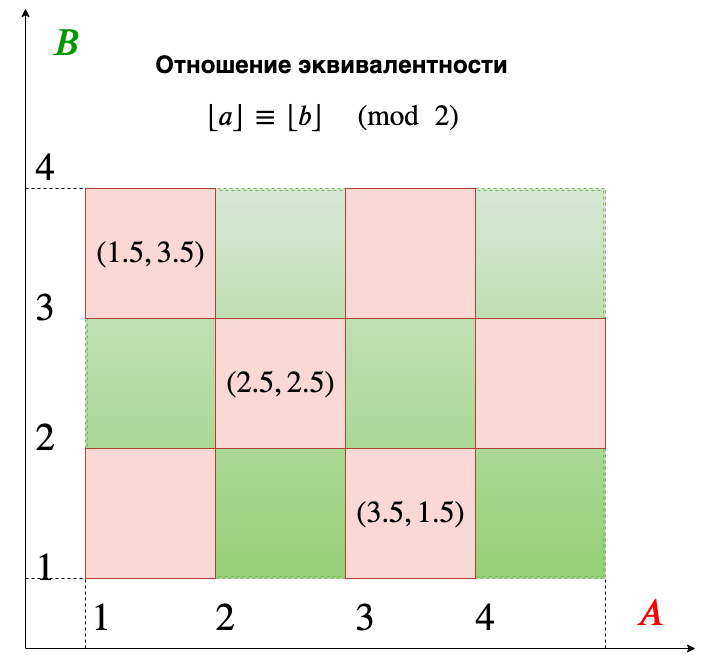
\includegraphics[scale=0.25]{equiv.png}
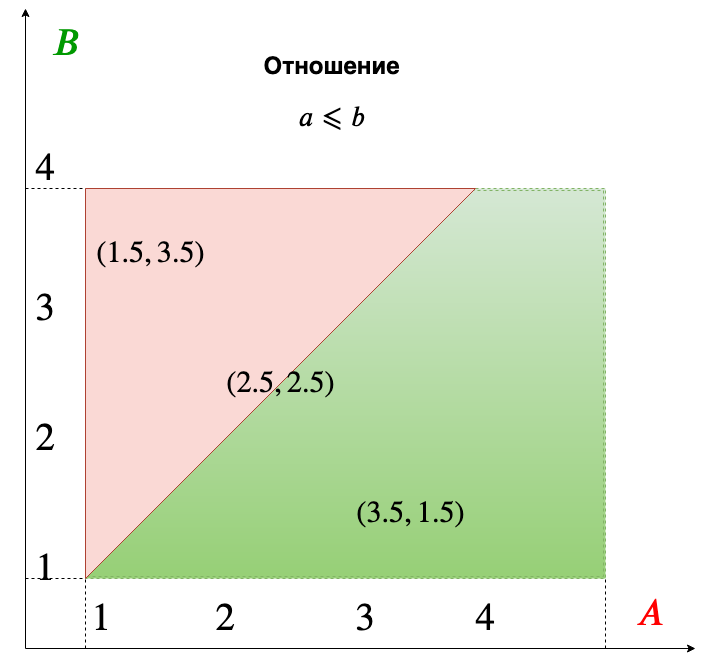
\includegraphics[scale=0.25]{lessthan.png}
\end{center}


\section{Числа Гаусса}

\subsection{Конспект}
\begin{enumerate}\setlength{\itemsep}{1pt}
\item 
\item 
\item 
\item 
\item 
\item 
\item 
\item 
\item 
\item 
\end{enumerate}
\subsection{Задачи}


\chapter{Линейные уравнения}

\section{Уравнение прямой на плоскости}

\subsection{Конспект}

\begin{enumerate}
\item Рассмотрим плоскость с координатными осями $Ox$ и $Oy$. Что будет, если ее начать поворачивать? Во что переходит при этом ось $Ox$?
\item Поскольку вращение --- это движение, расстояние между точками сохраняется, и значит, никакие три точки, лежащие на прямой $Ox$, при повороте не могут перейти в точки, образующие невырожденный треугольник --- они снова лягут на прямую, причем в том же самом порядке. Стало быть, $Ox$ при вращении плоскости переходит в некоторую прямую.
\item Пусть центорм вращения является точка $O=(0,1)$, и ось $Ox$ при вращении $R_\ph$ переходит в прямую $l$. Ясно, что $l$ такаже проходит через начало координат $O$, т.к. это --- стационарная точка вращения.
\item Фиксируем на $Ox$ точку $(1,0)$ и посмотрим, куда она переходит под действием всех возможных вращений. Поскольку расстояние от центра вращения сохраняется, ясно, что эта точка остается на окружности радиуса 1. В то же время, выбирая произвольную точку на этой окружности, мы легко укажем угол $\ph$, на который нужно осуществить поворот плоскости относительно центра $O$, чтобы точка $(1,0)$ перешла в выбранную нами точку.
\item Итак, под действием группы вращений точка $(1,0)$ переходит во все точки единичной окружности. Аналогично, если мы выберем произвольную точку $(r,0)$ ($r>0$), она будет переходить во все точки окружности радиуса $r$ под действием группы вращений с центром в точке $O$.
\item В этом случае принято говорить, что группа вращений \textbf{действует} на плоскости, а множество всех значений, в которые она переводит выбранную точку, называют \textbf{орбитой} этой точки. В нашем примере орбитами являются коцентрические окружности с центром $O$.
\item Можно доказать, что орбиты образуют классы экивалентности, т.е. они попарно не пересекаются и в сумме дают всю область действия группы.
\item Фиксируем некоторое вращение $R_\ph$, и пусть точка $(0,1)$ при таком вращении перешла в точку $C=(x_0,y_0)$, лежащую на единичной окружности.
\item Возьмем произвольную точку $(r,0)$, где $r>0$, и проследим ее судьбу под действием того же вращения $R_\ph$. Пусть $A=(x,y)=R_\ph(r,0)$. Ясно, что точки $O,C,A$ лежат на одной прямой $l$.
\item Проведем вертикальные линии через абсциссы $x_0$ и $x$, а также горизонтальные линии через ординаты $y_0$ и $y$. Добавим новые точки пересечения $B$ и $D$ (см. рисунок).

\begin{center}
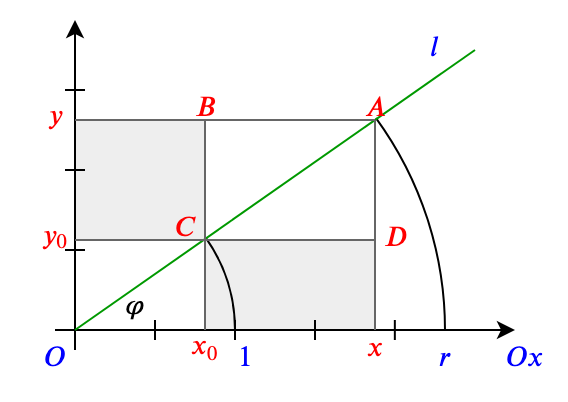
\includegraphics[scale=0.5]{linerotation.png}
\end{center}
\item Видим, что треугольники $ABC$ и $ADC$ равны по трем сторонам, также равны треугольники $Oy_0C$ и $Ox_0C$, и треугольники $OyA$ и $OxA$. Отсюда легко установить равенство площадей $x_0(y-y_0)=y_0(x-x_0)$, откуда получаем
$$
xy_0-yx_0=0.
$$
\item Поскольку $(x,y)$ --- это произвольная точка прямой $OC$ (для отрицательного $r$ все доказывается аналогично),  данное уравнение есть уравнение прямой, проходящей через начало координант с углом наклона $\ph$.
\item Отметим, что точка $(x_0,y_0)$ полностью определяется углом поворота $\ph$, т.к. является образом точки $(0,1)$ при повороте на угол $\ph$. В то же время, произвольная точка на единичной окружности однозначно задает угол поворота в интервале от 0 до $2\pi$. Таким образом, задать поворот с центром $O$ и задать точку на единичной окружности --- суть одно и то же.
\item Зная тригонометрию, можно также заметить, что $x_0=\cos\ph$ и $y_0=\sin\ph$, а отношение $y_0/x_0=\tan\ph$.
\item Кроме того, отношение $y_0/x_0$ также однозначно определяет угол поворота, но только в интервале от 0 до $\pi$.
\item Наконец, поворот прямой(!) на угол $\pi+\al$ --- это поворот на угол $\al$ с последующим отражением прямой $l$ относительно точки $O$. Но отражение прямой относительно своей же точки дает нам ту же самую прямую с тем же самым уравнением для ее точек! Таким образом, прямая, проходящая через начало координат полностью определяется тангенсом угла наклона, т.е. отношением $y_0/x_0$.
\item Но раз все дело в отношении, стало быть, прямая задается любой точкой, координаты которой находятся в таком же соотношении, что и коодинаты точки $(x_0,y_0)$, лежащие на единичной окружности. Иначе говоря, одну и ту же прямую задают также точки вида $(-x_0,-y_0)$, $(rx_0,ry_0)$, $(-rx_0,-ry_0)$, если коэффициент $r>0$. На рис. мы обозначили эти точки, соответственно, $C,A$ и $-C,-A$.
\begin{center}
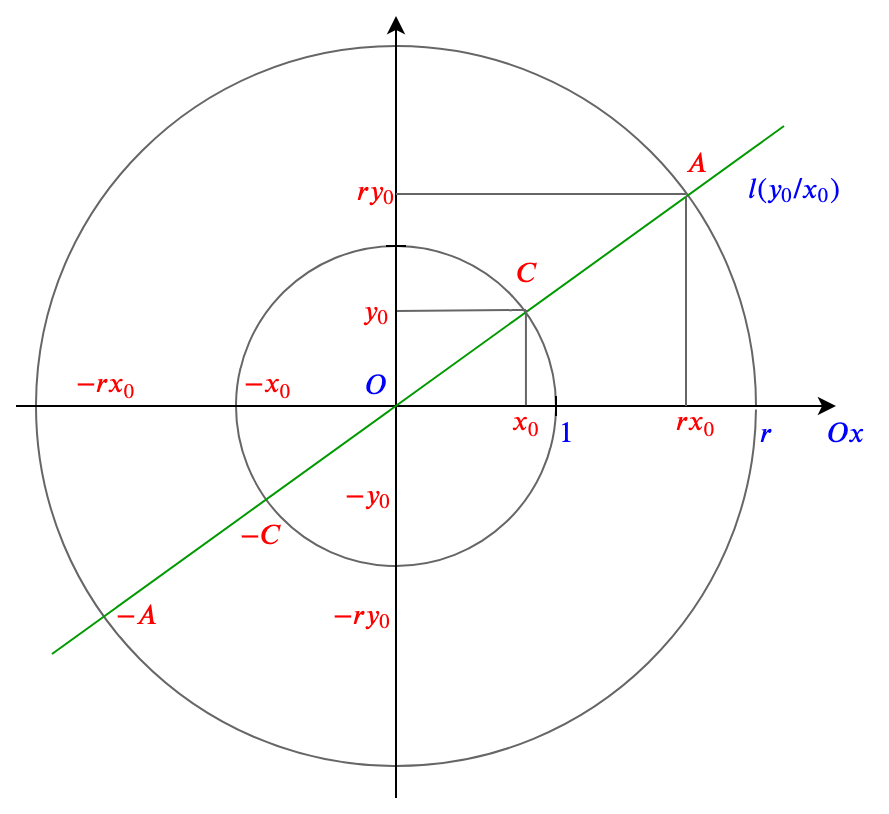
\includegraphics[scale=0.3]{line.png}
\end{center}
\item Этот вывод можно получить и более формально, просто глядя на уравнение прямой
$$
xy_0-yx_0=0.
$$
Ведь если мы домножим обе части уравнения на $r$, ничего не изменится!
$$
x(ry_0)-y(rx_0)=0.
$$
\item Что если прямая $l$ не проходит через центр координат $O$? В этом случае мы можем сдвинуть ее на некоторый вектор так, чтобы произвольно выбранная точка этой прямой перешла в точку $O$. Обозначим эту точку на прямой $l$ за $S=(\De x,\De y)$, а сдвиг, соответственно, осуществим на вектор $(-\De x,-\De y)$.
\begin{center}
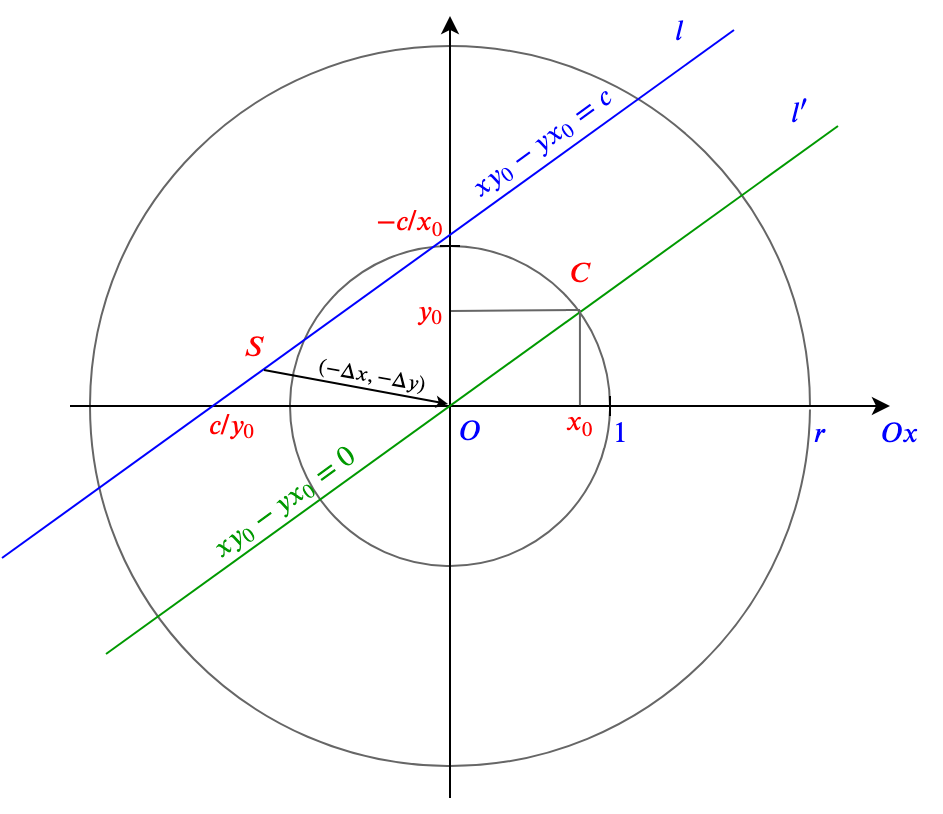
\includegraphics[scale=0.3]{lineshift.png}
\end{center}
\item Тогда смещенные координаты $(x-\De x,y-\De y)$ уже будут пробегать прямую $l'$, проходящую через центр $O$, а ее уравнение нам известно:
$$
(x-\De x)y_0 - (y-\De y)x_0=0,
$$
или
$$
xy_0-yx_0=c,\quad\mbox{где } c= y_0\De x - x_0\De y.
$$
При этом коэффициенты $(x_0,y_0)$ все так же отвечают за наклон прямой $l$ и полностью определяются тангенсом угла наклона прямой $l$ относительно положительного направления $Ox$, т.е. отношением $y_0/x_0$.
\item Может показаться, что уравнение сильно зависит от выбора точки $S$, поскольку слагаемое $c$ зависит от координат точки $S$. Покажем, что это не так. Пусть $S'=(\De x',\De y')$ --- какая-то другая точка прямой $l$. Но в этом случае она удовлетворяет найденному уравнению, т.е.
$$
\De x'y_0-\De y'x_0=c,
$$
но уравнение, найденное с помощью точки $S'$ будет иметь вид
$$
xy_0-yx_0= y_0\De x' - x_0\De y',
$$
откуда из предыдущего получаем, что вновь
$$
xy_0-yx_0=c.
$$
\item Таким образом, для нахождения $c$ мы можем выбрать любую понравившуюся нам точку прямой $l'$, например, отчку пересечения с одной из координатных осей.
\item В случае, когда $x_0\ne 0$, уравнение прямой можно переписать в виде
$$
y  = ax+b,\quad\mbox{где }a=\frac{y_0}{x_0},\; b=-\frac{c}{x_0}.
$$
В случае $x_0=0$ мы имеем вертикальную прямую $x=c$ (при угле $\ph=\pi/2$ мы получим $y_0=1$).
\end{enumerate}
\subsection{Задачи}

\begin{enumerate}
\item В какие точки переходят точки $(0,3)$ и $(4,0)$ при повороте на $90$ градусов? На $-90$ градусов?
\item Каков угол поворота, если точка $(a,b)$ перешла в точку $(-a,-b)$? В точку $(-b,a)$? В точку $(b,-a)$?
\item Чему равен тангенс угла наклона прямой $3x-5y=7$?
\item Какой угол наклона у прямой $y=-x+3$?
\end{enumerate}


\section{Линейные уравнения в целых числах}

\subsection{Конспект}

\begin{enumerate}
\item Поскольку мы пока владеем аппаратом только целых чисел (множество $\Z$), рассмотрим задачу о нахождении всех целых точек плоскости, через которые проходит заданная прямая. Под целыми точками плоскости мы будем понимать такие точки, координаты которых принадлежат $\Z$.
\item В общем виде \textbf{линейное уравнение в целых числах} выглядит следующим образом:
$$
ax-by=c,\quad\mbox{где коэффициенты } a,b,c\in\Z.
$$
Задача: найти все такие $x,y$, тоже целые, которые удовлетворяют данному уравнению.
\item Сначала рассмотрим случай т.н. \textbf{однородного уравнения}:
$$
ax-by=0,
$$
т.е. мы отбрасываем ту часть уравнения, которая не зависит от переменных $x,y$.
\item Как мы уже знаем, данное уравнение задает прямую, проходящую через начало координат, а ее наклон определяется отношением $a/b$.
\item Для начала проверим, нельзя ли данное отношение упростить. Если числа $a,b$ имеют какой-то общий делитель, то разумно было бы на него сократить. И чтобы не проверять это много раз, сократим их сразу на $\gcd(a,b)$. Множество решений от этого не изменится, а само уравнение по-прежнему останется однородным и целочисленным:
$$
\tilde ax-\tilde by=0,\quad\mbox{где } \tilde a=\frac{a}{\gcd(a,b)},\;\tilde b=\frac{b}{\gcd(a,b)}.
$$
\item Таким образом, мы приходим к уравнению со взаимно простыми коэффициентами $\tilde a$ и $\tilde b$.
\item Перепишем уравнение иначе: $\tilde ax=\tilde by$. Заметим, что все числа здесь --- целые. Причем $\tilde by$ делится на $\tilde a$. Но так как $\tilde a$ и $\tilde b$ взаимно просты, то $y$ делится на $\tilde a$. Это есть следствие того факта, который мы доказывали ранее в разделе \ref{PrimeNumbers}: если простое число $p$ делит произведение $ab$, то оно делит $a$ или $b$ (или их обоих). Поэтому если простое $p$ делит $\tilde a$, то оно делит $\tilde by$, но оно не может делить $\tilde b$, т.к. $\gcd(p,\tilde b)=1$, значит, оно делит $y$. Это значит, что все простые, составляющие число $\tilde a$, являются делителями $y$. В то же время, эти простые не входят в $\tilde b$, поскольку $\gcd(\tilde a,\tilde b)=1$. Поэтому, если $p^\al$ входит в разложение $\tilde a$, то $p^\al$ также делит $y$. Следовательно, $y$ делится на $\tilde a$, т.е. 
$$
y=k\tilde a
$$
при некотором целом $k$.
\item Симметрично рассуждая, получаем, что $x$ делится на $\tilde b$, т.е.
$$
x=t\tilde b
$$
при некотором целом $t$.
\item Подставим эти выражения в наше однородное уравнение:
$$
\tilde a(t\tilde b)=\tilde b(k\tilde a),
$$
откуда
$$
t=k,
$$
и больше никаких ограничений на выбор коэффициента $k$ мы не имеем.
\item Таким образом, решениями уравнения $\tilde ax-\tilde by=0$ являются
$$
\begin{cases}
x  =k\tilde b=kb/\gcd(a,b), \\
y  =k\tilde a=ka/\gcd(a,b),
\end{cases}
$$
где $k\in\Z$. Эти же $x$ и $y$ являются решениями исходного однородного уравнения $ax-by=0$.
\item Вернемся к неоднородному уравнению $ax-by=c$.
\item Для начала заметим, что если данное уравнение имеет решение в целых числах, то $ax-by$ делится на $\gcd(a,b)$, а значит, $c$ делится на $\gcd(a,b)$. Поэтому, если $c$ не делится на $\gcd(a,b)$, то решений точно нет, т.е. в таком случае прямая $ax-by=c$ проходит мимо всех целых точек плоскости!
\item Покажем, что в случае делимости $c$ на $\gcd(a,b)$ решения обязательно есть, и опишем все такие решения.
\item Пусть $c=d\gcd(a,b)$.
\item В разделе \ref{PrimeNumbers} мы установили, что $\gcd(a,b)$ является линейной комбинацией чисел $a$ и $b$, т.е.
$$
\gcd(a,b) = an-bm
$$
при некоторых целых $n$ и $m$ (понятно, что знак перед $m$ можно выбирать любой, поэтому выберем так, как нам удобнее).
\item Отсюда следует, что пара чисел $(dn,dm)$ удовлетворяет уравнению $ax-by=c$, поскольку
$adn-bdm=d\gcd(a,b)=c$.
\item Итак, представив $\gcd(a,b)$ в виде линейной комбинации $a$ и $b$, мы можем найти одно решение исходного уравнения.
\item Далее применим тот же прием, что и при изучении уравнений прямых --- сдвинем прямую $ax-by=c$ так, чтобы точка $(dn,dm)$ оказалась в начале координат. Для этого введем новые переменные
$$
\hat x = x-dn,\quad \hat y = y-dm.
$$
\item Тогда получаем, что $a\hat x-b\hat y = 0$. А такое уравнение мы уже решили выше, и его решением будет пара чисел $\hat x = kb/\gcd(a,b)$ и $\hat y = ka/\gcd(a,b)$, где $k$ --- любое целое число.
\item Собирая все вместе, находим общее решение исходного уравнения:
$$
\begin{cases}
x  =kb/\gcd(a,b) + dn, \\
y  =ka/\gcd(a,b) + dm,
\end{cases}
$$
\item Таким образом, решением линейного уравнения $ax-by=c$ в целых числах является сумма общего решения однородного уравнения $ax-by=0$ и какого-нибудь частного решения исходного уравнения.
\item Основной трудностью при поиске частного решения является нахождение коэффициентов $n$ и $m$ представления $\gcd(a,b)$.
\item Это представление можно найти с помощью алгоритам Евклида. Рассмотрим для примера уравнение
$$
18x-11y=2
$$
\item Следуя алгоритму Евклида, получаем выкладки:
\begin{align*}
18 = & 11\cdot 1+7,\\
   & 11 = 7\cdot 1 + 4, \\
   & 7 = 4\cdot 1 + 3, \\
   & 4 = 3\cdot 1 + 1
\end{align*}
Последняя 1 --- это и есть $\gcd(18,11)$. Раскрутим алгоритм в обратную сторону:
\begin{align*}
1 & = 4-3 = 4 - (7-4) = 4\cdot 2-7 = (11-7)\cdot 2-7 =\\
  & = 11\cdot 2-7\cdot 3 = 11\cdot 2 - (18-11)\cdot 3 =\\
  & = 11\cdot 5 - 18\cdot 3.
\end{align*}
Таким образом, наши искомые числа $n=-3$, $m=-5$. Напомним, что мы ищем представление $\gcd(18,11)$ в виде $18n-11m$, исходя из чего нужно правильно выбирать знаки перед коэффициентами.

Кроме того, $d=2$, т.к. $c=2$ и $\gcd(a,b)=1$. Откуда общее решение уравнения $18x-11y=2$ получаем в виде:
$$
\begin{cases}
x  =11k - 6, \\
y  =18k - 10,
\end{cases}
$$
где $k$ --- любое целое число. Проверим:
$$
18(11k - 6) - 11(18k - 10) = 198k-198k - 108 + 110 =2.
$$
\item Наконец, приведем еще один замечательный способ найти разложение НОД. Этот метод основан на представлении дробей в виде т.н. \textbf{цепных дробей}. Пусть дано уравнение
$$
112x-34y=16.
$$
\item Ищем приближение дроби $112/34$ следующим способом:
$$
\frac{112}{34} = 3 + \frac{5}{17} = 3 + \frac{1}{3+\frac{2}{5}} = 
3 + \frac{1}{3 + \frac{1}{2+1/2}}
$$
По сути дела, это --- другая запись выкладок алгоритма Евклида, поскольку мы каждый раз последовательно выделяем неполное частное предыдущих остатков.

Как только мы дошли до хвоста вида $1/k$, мы останавливаемся, отбрасываем этот хвост и сворачиваем дробь обратно, получая приближение исходной дроби:
$$
\frac{112}{34} \approx 3 + \frac{5}{17} = 3 + \frac{1}{3+\frac{2}{5}} = 
3 + \frac{1}{3 + \frac{1}{2}} = \frac{23}{7}
$$
Далее, перемножая накрест эти дроби, получаем представление для НОД:
$$
\gcd(112,34) = 112\cdot 7 - 34\cdot 23.
$$
Искомые коэффициенты: $n=7$, $m=23$. Общее решение уравнения, таким образом, получаем в виде
$$
\begin{cases}
x  = 34k +  8\cdot 7, \\
y  = 112k + 8\cdot 23 ,
\end{cases}
$$
где $k$ --- любое целое число, а $8=16/\gcd(112,34)$. Проверяем:
$$
112(34k +  8\cdot 7)-34(112k + 8\cdot 23) = 8(112\cdot 7- 34\cdot 23) = 16.
$$
\item Выше мы всюду рассматривали уравнения, в которых $x$ идет с положительным коэффициентом, а $y$ --- с отрицательным. Иначе говоря, прямая, заданная таким уравнением, имеет наклон <<вправо>>. Но уравнение может быть, например, таким
$$
5x+9y=1.
$$
Если мы хотим решать его по тем же формулам, то лучше перейти к новым переменным $\hat x=x$, $\hat y=-y$, и тогда мы получим уравнение
$$
5\hat x-9\hat y=1.
$$
Найдя его решения, мы просто меняем знак у $\hat y$, и получаем исходное уравнение.
\end{enumerate}

\subsection{Задачи}

\begin{enumerate}
\item Найти представление $\gcd(5,9)$ с помощью алгоритма Евклида и методом цепных дробей.
\item Найти представление $\gcd(18,15)$ с помощью алгоритма Евклида и методом цепных дробей.
\item Найти представление $\gcd(225,81)$ с помощью алгоритма Евклида и методом цепных дробей.
\item Решить уравнение $5x-9y=2$ в целых числах.
\item Найти все решения уравнения $225x+81y=18$ в целях числах.
\item Найти все решения уравнения $10x-18y=3$ в целях числах или доказать, что их нет.
\end{enumerate}



\chapter{Числовые поля}

\section{Рациональные числа}

\subsection{Конспект}
\begin{enumerate}
\item Предыдущую главу мы закончили действиями с дробями, хотя нигде до сих пор о них не говорили. Разве что, упоминали отношение $y_0/x_0$ как некоторый параметр, определяющий угол наклона прямой на координатной плоскости.
\item Итак, рассмотрим прямую $l$, заданную уравнением $ax-by=0$, где $a,b$ --- целые числа.
\item Для начала пусть $a=1$ и $b>1$. Легко видеть, что такая прямая проходит через точки $(0,0)$ и $(b,1)$ (см. рис.).
\begin{center}
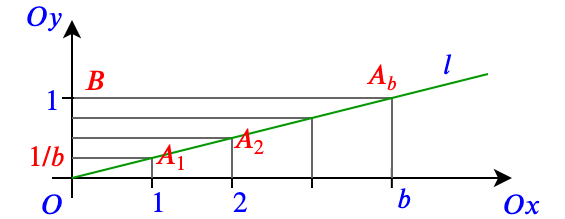
\includegraphics[scale=0.5]{section.png}
\end{center}
\item На прямой $l$ мы можем поставить точки $A_1, A_2, \dots, A_b$ в местах пересечения этой прямой с вертикальными прямыми, имеющими уравнения $x=1, x=2, \dots, x=b$, соответственно.
\item Теперь рассмотрим треугольник $OBA_b$, где точка $B=(0,1)$. В этом треугольнике мы можем провести линии, параллельные его горизонтальной стороне $BA_b$, которые отсекут на вертикальной стороне $OB$ нашего треугольника отрезки.
\item Эти отрезки будут иметь одинаковую длину по теореме Фалеса, т.к. точки на прямой $l$ также расставлены с одинаковым шагом, что следует уже из выбора вертиклаьных секущих (они идут с шагом 1).
\item Итак, мы вертикальной оси мы получили $b$ одинаковых отрезков, сумма длин которых равна 1.
\item Какова же длина каждого из таких отрезков? Ответ: она равна одной $b$-ой части единицы. И эта часть записывается как дробь $1/b$. Собственно, отношение $1/b$, как мы видели ранее, является определяющим для прямой $l$.
\item Мы можем брать сумму нескольких таких частей, например, $k$ частей размера $1/b$ дают в сумме отрезок длины в $k$ раз больше, чем отрезок $1/b$. Такая часть записывается в виде дроби $k/b$.
\item Величину $k/b$ можно получить иным способом. Возьмем теперь прямую $l'$, заданную уравнением $kx+by=0$ (см. рис.).
\begin{center}
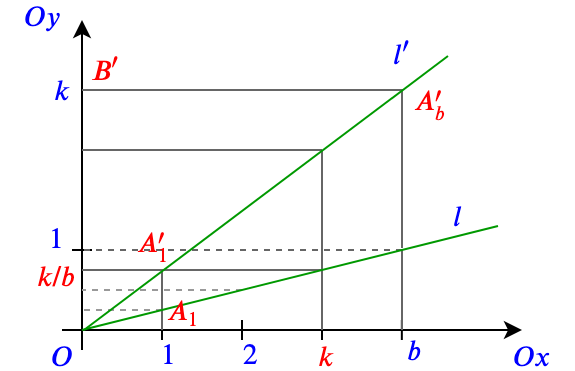
\includegraphics[scale=0.5]{sectionkb.png}
\end{center}
\item Эта прямая проходит через начало координат и точку $(b,k)$.
\item Проделаем аналогичные предыдущему построения: проведем вертикальные линии с шагом 1, а затем горизонтальные линии от точек пересечения вертикальных с прямой $l'$, и посмотрим, какие отрезки у нас полуучатся на оси $Oy$.
\item Нетрудно видеть, что линия, соответствующая $x=k$, для прямой $l$ отсекает на оси $Oy$ метку, которую мы обозначили как $k/b$. Но ровно ту же самую метку покажет построение с помощью вертикальной линии $x=1$ и прямой $l'$. Почему? А очень просто: достаточно сравнить уравнения этих прямых
$$
l:\;x-by=0,\quad l':\;kx-by=0.
$$
\item Если в первом вместо $x$ подставить $k$, а во втором вместо $x$ подставить 1, то получим одно и то же значение $y$. Отсюда и совпадение меток.
\item Таким образом, прямая $l'$ дает на оси $Oy$ шаг в $k$ раз больше, чем прямая $l$, если мы строим сечения при одном и том же $x$ (не обязательно $x=1$).
\item Получается, что прямая, заданная уравнением $kx-by=0$, задает умножение на число $k$ всех чисел, получаемых прямой, заданной уравнением $x-by=0$.
\item Рассматривая эти прямые как некие новые объекты, мы можем ввести понятие умножения прямой на целое число. Если у нас есть прямая $ax-by=0$, то результатом ее умножения на число $k$ является прямая $kax-by=0$. Запишем это так:
$$
k(ax-by=0) = (ka)x-by=0.
$$
\item Заметим, что сложение (и вычитание) таких прямых определить еще проще: 
$$
(a_1x-by=0)+(a_2x-by=0) = ((a_1+a_2)x-by=0).
$$
\item Все прямые вида $ax-by=0$ при фиксированном $b\ne 0$ с определенныими выше операциями сложения и умножения образуют кольцо. 
\item Если вместо сложной записи $ax-by=0$, описывающей прямую, записать просто отношение $a/b$, то мы увидим, что операции с прямыми образуют в точности операции с дробями:
$$
k\frac{a}{b}  = \frac{ka}{b}\quad\mbox{и}\quad\frac{a_1}{b}+\frac{a_2}{b} = \frac{a_1+a_2}{b}.
$$
\item Заметим теперь, что уравнение $x-by=0$ прямой $l$ можно переписать иначе: $kx-(bk)y=0$. Чем оно отличается от уравнения $kx-by=0$ прямой $l'$? Очевидно, тем, что перед $y$ появился коэффициент $k$. А тепрь вспомним, что прямая $l$ задает отношение в $k$ раз меньше, чем прямая $l'$! И это значит, что если мы хотим разделить прямую $l'$ на $k$, то мы должны умножить на $k$ ее коэффициент перед $y$.
\item Итак, если мы хотим умножить прямую на число, то мы умножаем на это число коэффициент перед $x$ (прямая становится более крутой), а если мы хотим разделить прямую на число, то мы умножаем на это число коэффициент перед $y$ (прямая становится более пологой).
\item Делаем следующий шаг: умножение двух прямых. На самом деле, любую прямую $ax-by=0$ мы можем переписать как серию ранее определенных операций:
$$
(ax-by=0) = a(x-y=0)/b,
$$
при этом прямая $x-y=0$ имеет наклон 45 градусов и соответствует отношению 1/1, т.е. по-просту 1, и в операциях умножения может опускаться. Таким образом, умножени прямых выглядит следуюим образом
\begin{gather*}
(a_1x-b_1y=0)(a_2x-b_2y=0) = \\
= a_1(x-y=0)/b_2\cdot a_2(x-y=0)/b_2 = (a_1a_2x-b_1b_2y=0),
\end{gather*}
а это в точности умножение дробей: $(a_1/b_1)(a_2/b_2) = (a_1a_2)/(b_1b_2)$.
\item Отсюда нетрудно получить и процедуру деления прямых друг на друга:
$$
(a_1x-b_1y=0)/(a_2x-b_2y=0) = ((a_1b_2)x-(a_2b_1)y=0),
$$
что соответствует операции с дробями:
$$
\frac{a_1}{b_1}/\frac{a_2}{b_2} = \frac{a_1b_2}{a_2b_1}.
$$
\item Наконец, чтобы научиться складывать произвольные прямые, мы должны уметь сводить сложение произвольных прямых к сложнию прямых с одинаковым коэффициентом перед $y$, т.к. сложение мы определили выше только для данного случая.
\item Но и это не проблема:
\begin{gather*}
(a_1x-b_1y=0)+(a_2x-b_2y=0) = (a_1b_2x-b_1b_2y=0) + (a_2b_1x-b_1b_2y=0) = \\
= ((a_1b_2+a_2b_1)x-(b_1b_2)y=0),
\end{gather*}
что соответствует операциям с дробями
$$
\frac{a_1}{b_2}+\frac{a_2}{b_2} = \frac{a_1b_2+a_2b_1}{b_1b_2}.
$$
\item В целом картина представления рациональных чисел с помощью прямых с целочисленными коэффициентами выглядит следующим образом:
\begin{center}
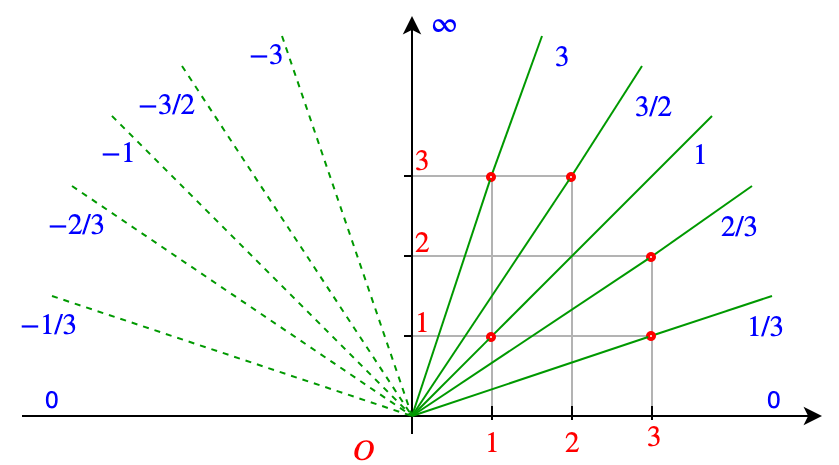
\includegraphics[scale=0.4]{ratio.png}
\end{center}

\item Итак, имея только множество целых чисел $\Z$, мы построили на плоскости всевозможные прямые, заданные линейными уравнениями с целыми коэффициентами, научились их складывать, вычитать, умножать и делить. Тем самым, мы построили новую алгебраическую структуру, которая называется \textbf{полем}. Поле --- это кольцо, в котором можно делить на любое число, кроме нуля.
\item Записывая эти прямые не уравнениями, а отношением коэффициентов (вместо $ax-by=0$ пишем $a/b$), мы получаем \textbf{поле рациональных чисел}, которое принято обозначать $\Q$.
\item На самом деле, в нашем построении есть еще и такая прямая, которая соответствует бесконечности. Это прямая, заданная уравнением $x=0$. А нулевая прямая определяется уравнением $y=0$. В полном соответствии с установленными правилами, мы можем заметить, что
\begin{gather*}
(ax-by=0)(y=0)=(y=0),\;(ax-by=0)(x=0)=(x=0),\\ 
(ax-by=0)/(y=0)=(x=0),\;(ax-by=0)/(x=0)=(y=0),
\end{gather*}
т.е. деление на ноль дает бесконечность, а деление на бескончность дает ноль, и т.д.
\item Тем не менее, в обычном поле такие исключительные элементы не обязательны, и поэтому деление на ноль не постулируется.

\end{enumerate}


\subsection{Задачи}


\section{Многочлены}
\subsection{Конспект}
\begin{enumerate}\setlength{\itemsep}{1pt}
\item 
\item 
\item 
\item 
\item 
\item 
\item 
\item 
\item 
\item 
\end{enumerate}
\subsection{Задачи}

\begin{comment}

81-82
https://www.youtube.com/watch?v=JM_7-JcD4IQ
00-00 кузнечик с ногами 1 и альфа
2-30 альфа - иррациональная => слепых зон нет
3-50 всюду плотное множество
4-40 доказательство. Всю прямую наматываем на окружность
12-50 для любого эпсилон можно найти точки кратные альфа в пределах эпсилон, сколь угодно малого
13-10 доказательство от противного
18-30 иррациональные числа бывают разные
20-20 приделаем кузнечику еще одну ногу альфаквадрат
29-00 степень алгебраического числа
32-50 подход 1, альфа алгебраическое, если существует многочлен с целыми коэф
34-30 второй подход
37-00 многочлен самой маленькой степени, как вычислить?
39-30 доказательство что корень кубической степени из двух имеет степень 3
40-00 ступень 1
41-10 ступень 2 (лемма Гаусса)
45-00 ступень 3
47-00 докажем ступень 3
57-00 докажем ступень 1
1-05-00 что если в общем случае (а не корень кубический из 2)
1-09-00 многочлен нечетной степени всегда имеет корень
\end{comment}


\section{Рациональные числа}

\subsection{Конспект}
\begin{enumerate}\setlength{\itemsep}{1pt}
\item 
\item 
\item 
\item 
\item 
\item 
\item 
\item 
\item 
\item 
\end{enumerate}
\subsection{Задачи}


\begin{comment}

19-20
2015_10_28 - 19-я и 20-я лекция д. ф.-м.н. А. В. Савватеева ч. ⅛
https://www.youtube.com/watch?v=m_N1Jc3HapU

2-30 соизмеримость отрезков
4-00 алгебраическая запись а=md b=nd
6-50 соотношение отрезков - рациональное число ⇔ соизмеримость

2015_10_28 - 19-я и 20-я лекция д. ф.-м.н. А. В. Савватеева ч. 2/8
https://www.youtube.com/watch?v=PsAxdahrv1Q

0-00 что если а и в несоизмеримы?
1-20 задача про кузнечика
2-50 ах+ву=с, а=корень из двух, в=1, сложное множество
6-00 если соизмеримы, то…
9-00 d(НОД(mn)z)

2015_10_28 - 19-я и 20-я лекция д. ф.-м.н. А. В. Савватеева ч. ⅜
https://www.youtube.com/watch?v=po68il5wqp0

1-30 все кратные отрезка d*НОД(mn)

2015_10_28 - 19-я и 20-я лекция д. ф.-м.н. А. В. Савватеева ч. 4/8
https://www.youtube.com/watch?v=9z8reMyp8ls

0-00 НОД (17 12)
2-00 геометрическая иллюстрация 17 на 12

2015_10_28 - 19-я и 20-я лекция д. ф.-м.н. А. В. Савватеева ч. ⅝
https://www.youtube.com/watch?v=Wi4R9Y-0XsI

0-00 геометрический алгоритм Евклида

2015_10_28 - 19-я и 20-я лекция д. ф.-м.н. А. В. Савватеева ч. 6/8
https://www.youtube.com/watch?v=vE6lFlpaVcE

0-00 цепные дроби 17/12
3-00 три ипостаси одного и того же
6-00 пишем любую цепную дробь

2015_10_28 - 19-я и 20-я лекция д. ф.-м.н. А. В. Савватеева ч. ⅞
https://www.youtube.com/watch?v=pHhQ_xoT1gA

Проверяем цепную дробь
Феномен цепных дробей - дроби с отличием на 1

2015_10_28 - 19-я и 20-я лекция д. ф.-м.н. А. В. Савватеева ч. 8/8
https://www.youtube.com/watch?v=xUPSD4zOPOM


0-00 ad-bc=+-1 GL2(Z)
2-00 кузнечик с соизмеримыми отрезками
3-00 геометрическое представление
7-00 "... словами и так до бесконечности!"
\end{comment}


\section{Цепные дроби}

\subsection{Конспект}
\begin{enumerate}\setlength{\itemsep}{1pt}
\item 
\item 
\item 
\item 
\item 
\item 
\item 
\item 
\item 
\item 
\end{enumerate}
\subsection{Задачи}



\section{Расширение поля рациональных чисел}




\subsection{Конспект}
\begin{enumerate}\setlength{\itemsep}{1pt}
\item 
\item 
\item 
\item 
\item 
\item 
\item 
\item 
\item 
\item 
\end{enumerate}
\subsection{Задачи}

\begin{comment}

93-94
Вещественные числа: аксиома полноты
https://www.youtube.com/watch?v=1GAIDF8TPYQ
00-00 аксиома полноты, вещественные числа
1-00 в любой ли точке живет число?
3-00 алгоритм нахождения любого числа/точки
6-50 соответствие N и R
11-50 на прямой есть точки к которым можно обратиться только аз бесконечное количество итераций
13-20 любая последовательность вложенных отрезков имеет непустое пересечение
14-30 последовательность приближений
16-00 Любая монотонная ограниченная последовательность имеет предел
18-30 монотонность
20-30 ограниченность
25-30 предел монотонной последовательности
31-00 последовательность вычисления корня
33-00 определение предела
41-00 последовательность, которая обращается к числам
42-00 определить поведение последовательности
42-30 определение Коши
47-00 как учат матан в плохом вузе
48-00 А3: любая фундаментальная последовательность имеет предел
50-30 подходы к исследованию отсутствия дыр :)
52-00 последовательность n^k/2^n
54-00 экспонента забивает степенную
55-00 последовательность a^n/n!
58-00 подмножество R - ограничено если…
59-00 уточнение: ограничено сверху, если..
1-00-00 ограничено снизу, если…
1-01-00 идея полноты
1-03-30 верхняя грань множества А
1-09-00 модель вещественных чисел
1-12-30 человечество пришло к вещественным числам 150 лет назад
1-15-00 Сечение Дедекинда

95-96
сечения Дедекинда и другие модели вещественных чисел
https://www.youtube.com/watch?v=eFIWK1NVJcA
00-01 аксиомы чисел
2-30 ответы начинаются с Кантора: множества всех точек прямой больше чем натуральные
3-00 число по Д: множество рациональных, такое что…
6-00 какие сечения Д отвечают требованиям рациональных чисел?
13-00 очевидность заменяем на аксиому
13-30 для любого эпсилон, существует эн, что 1/n<e
16-00 что такое сумма двух чисел (сумма минковского раньше минковского)
17-40 нерешенная задача математики - об одновременном “падении” множеств
24-10 три аспекта вещественных чисел
25-10 коммутативная группа по сложению
26-00 группа по умножению
26-30 отдельно стоящий закон - распределитель
27-00 означает поле
27-05 упорядоченность поля
27-50 еще две аксиомы связанные с порядком
29-30 доказываем что 1>0
31-10 модель бесконечных -ичных дробей
37-00 почему 0,99999...999 в точности равно 1
38-50 сложение и умножение, выяснение числа какого-то разряда
40-00 сравнение последовательностей
42-10 теорема: точки отрезка 0-1  то же самое, что и последовательности 0 и 1 (без хвостов)
48-00 2^N=R
50-30 проблемы Гильберта
56-00 о корнях, существует ли?
1-00-00 теорема: корни корней корней... стремится к 1
1-10-00 о степенях
1-10-30 n^k/f^n=>0
1-15-00 зажимание последовательности двумя другими
1-16-30 a^n/n!
\end{comment}


\section{Вещественные числа}

\subsection{Конспект}
\begin{enumerate}\setlength{\itemsep}{1pt}
\item 
\item 
\item 
\item 
\item 
\item 
\item 
\item 
\item 
\item 
\end{enumerate}
\subsection{Задачи}


\section{Комплексные числа}

\subsection{Конспект}
\begin{enumerate}\setlength{\itemsep}{1pt}
\item 
\item 
\item 
\item 
\item 
\item 
\item 
\item 
\item 
\item 
\end{enumerate}
\subsection{Задачи}



\section{Реализация движений с помощью комплексных чисел}

\subsection{Конспект}
\begin{enumerate}\setlength{\itemsep}{1pt}
\item 
\item 
\item 
\item 
\item 
\item 
\item 
\item 
\item 
\item 
\end{enumerate}
\subsection{Задачи}



\section{Гомотетии прямой и плоскости}

\subsection{Конспект}
\begin{enumerate}\setlength{\itemsep}{1pt}
\item 
\item 
\item 
\item 
\item 
\item 
\item 
\item 
\item 
\item 
\end{enumerate}
\subsection{Задачи}




